%%This is a very basic article template.
%%There is just one section and two subsections.
\documentclass{article}

\usepackage{amsmath}
\usepackage{caption}
\usepackage{placeins}
\usepackage{graphicx}
\usepackage{subcaption}
\usepackage{tikz}
%\usepackage{mathabx} % for \widebar
%\usepackage[active,tightpage]{preview}
\usepackage{natbib}
\bibpunct{(}{)}{,}{a}{}{;} 
\usepackage{url}
\usepackage{nth}
\usepackage{authblk}
% for the d in integrals
\newcommand{\dd}{\; \mathrm{d}}
\newcommand{\tc}{\quad\quad\text{,}}
\newcommand{\tp}{\quad\quad\text{.}}
\defcitealias{HMD}{HMD}
\defcitealias{HFD}{HFD}
\usepackage[titletoc,title]{appendix}
\newcommand\ackn[1]{%
  \begingroup
  \renewcommand\thefootnote{}\footnote{#1}%
  \addtocounter{footnote}{-1}%
  \endgroup
}

% a more sensitive widebar
% code found here:
% http://tex.stackexchange.com/questions/16337/can-i-get-a-widebar-without-using-the-mathabx-package
\makeatletter
\newcommand*\rel@kern[1]{\kern#1\dimexpr\macc@kerna}
\newcommand*\widebar[1]{%
  \begingroup
  \def\mathaccent##1##2{%
    \rel@kern{0.8}%
    \overline{\rel@kern{-0.8}\macc@nucleus\rel@kern{0.2}}%
    \rel@kern{-0.2}%
  }%
  \macc@depth\@ne
  \let\math@bgroup\@empty \let\math@egroup\macc@set@skewchar
  \mathsurround\z@ \frozen@everymath{\mathgroup\macc@group\relax}%
  \macc@set@skewchar\relax
  \let\mathaccentV\macc@nested@a
  \macc@nested@a\relax111{#1}%
  \endgroup
}
\makeatother

% another table trick:
% allows for changing alignment of cells 
\newcommand*{\myalign}[2]{\multicolumn{1}{#1}{#2}}


\begin{document}


\title{Life lost, lifesaving, and causes of death.}

\author[1]{Tim Riffe\thanks{triffe@demog.berkeley.edu}}
\author[2]{A{\"i}da Sol\'{e} Aur\'{o}}
\affil[1]{Department of Demography, University of California, Berkeley}
\affil[2]{Universitat Pompeu Fabra}

\maketitle

% 
\begin{abstract}
The lives and potential years of life lost due to death are presented as a metric for describing the population impacts of death and for comparing causes of
death. Lost lives and years of life may be classified by the ages in which
deaths occurred, by the ages to which deaths would be postponed were they saved, by the
ages through which the lost years would have been lived, or by the distribution of
lost remaining lifespans. These temporal perspectives define the
potential impacts of death and causes of death on population size and structure,
and on the distribution of lifespans within populations. We
illustrate these concepts using 2010 all-cause and cause-specific death
data for the USA from the Human Mortality Database. \ackn{Research reported in this manuscript
was supported by the U.S.
National Institute On Aging of the National Institutes of Health under award numbers R01-AG011552 and R01-AG040245 and by the Spanish Ministry of Science and Innovation under award
number ECO2013-48326-C2-1-P. The content is solely the responsibility of the
authors and does not necessarily represent the official views of the funding
agencies.}
\end{abstract}

\section*{Introduction}
A core task of demography is to account for and predict the population
pyramid and the forces that shape it. The pyramid represents population
size and age-sex structure, and it is shaped by the flows of births,
deaths, and migrations\footnote{We are guilty of omitting migration from
the following exposition, although some of the methods presented here would
translate cleanly to emigration.}. Of these flows, births are usually regarded
as the primary driver of variation in the profile of the pyramid,\footnote{This
is true to the extent that wars, epidemics, and other mortality shocks effect
broad age ranges rather than abrupt age groups.} whereas the pattern of survival
exerts a gentler influence on the overall tapering and height of the pyramid.
Year to year variation in the number of deaths tends to deduct
smoothly from a wide range of ages, making all but the most
severe mortality shocks illegible in the pyramid. This could be one of the
reasons why relationships between mortality and age structure have been less charted than those between births and age structure.

Demographers most often quantify death in terms of age-specific rates via the
lifetable and its summary indices because these are considered purged of
accidental distortions from population age structure. Moreover, public health
institutions and news media often also report trends in absolute numbers of
deaths from particular causes and the total potential years of life lost (YPLL) due to these deaths.\footnote{\citet{gardner1990} review commonly used methods of
calculating YPLL. The Global Burden of Disease reports refer to YPLL as YLL.
As a news media example, in 2013 the Guardian ran a data blog entry
visualizing the years of life lost in the USA due to gun violence
\citep{rogers2013gun}. } The notion of YPLL dovetails with
population size over time. In either of these treatments, mortality and deaths are
isolated from age structure. 

The point of departure for this article is to
treat deaths analytically as population stocks through the notion of
potentially saveable life. A potentially saveable life is a life that
has been lost, a death, and a set of lost lives is a kind of population. The
population of lost lives has static characteristics observed at the moment of
death, such as age and sex structure. Were the
population still living, it would still be subject to a continued force of
mortality and therefore retain a structure of remaining lifespans.
Observed mortality patterns may be used to project remaining lifespan structure onto the lost population as an approximation of what would
happen were the population to be resurrected simultaneously. In other words, we
may estimate the vital momentum lost due to death. By hypothetically saving a
life, we also save its momentum. By defining a universe of saveable lives in
this way, we make no statement on the feasibility of lifesaving, but wish
rather to make statements on the quantitative importance of lifesaving, wherein
years of life are the universal currency.
This step is a counterfactual exercise, in line with the formal treatment given in \citet{vaupel1987repeated}.\footnote{\citet{vaupel2008lifesaving} follows in a similar vein, but aims at the effects of lifesaving on period distortions.} Saveable life and lifetime can be quantified under various demographic perspectives on age and lifespan. These perspectives refine and supplement YPLL when assessing the population impacts of causes of death, and we think that they would provide useful information for the targetting and planning of public health interventions and the comparison of mortality burdens between populations and subpopulations.

We first formally define what is meant by age and lifespan
perspectives, illustrating on the example of all-cause
mortality before proposing an extention to causes of death. Concepts are
illustrated based on the population of the United States in 2010 based on pre-release
data newly collected by the Human Mortality
Database~\citepalias{HMD}. We propose
a selection of strategies for visualizing and arranging results for purposes of
reporting or making comparisons. Finally we discuss the limits of these methods
and the utility of the information gained by them. All mortality data used in
the following comes from the HMD.

\section*{Temporal relationships: Age and lifespan perspectives}
% To begin, sume a closed population and ignore what determines the size of
% successive birth cohorts, $B(t)$, which we usually call the birth flow. If
% $B(t)$ is a given, then the only other factor that determines population size
% and age structure is the length of the lives of its members. For simplicity,
% assume that the age pattern to mortality is fixed (this isn't necessary, but
% it simplifies notation). The population of age $a$ in year $t$, $P(a,t)$, is a function of 
% the survival of the birth cohort born in year $t-a$. Since we're
% fixing mortality, survival from age 0 to $a$ is $l(a)$ for any given cohort,
% so $P(a,t) = B(t-a)l(a)$.

% AS: Temporal relationships: I really like this section, but I think it needs
% to be reordered. Starting from Figure 1, moving to Figure 2 which perfectly illustrates what you 
% can do (using different populations) to compute the average years of life
% left. But I suggest you to first describe the idea, what you have done at the
% bottom of page 2 and then say something like: "and this translates into the following 
% form"; therefore, you can add your formulas. Followed by Figure 3. Since I am
% writing this email as I am reading, I just realized that you need a paragraph in front to introduce
% what follows: a) lifetime; b) remaining years of life; c) potentially savable lives. I need to 
% think more about these figures, but the work is there.  

Population stock in a
 given year, $t$, can be structured by birth cohorts or age, the way we typically make 
 population pyramids. If an entire lifespan is denoted by the random variable
 $X$, then the remaining lifespan, $y$, of a still-alive person aged $a$, $y = X - a$.
\begin{figure}[h]
% Figure produced in R/LifeLine.R
\centering
	\caption{A lifeline, where chronological age (years lived) is indexed by $a$
	and thanatological age (years left) is indexed by $y$.}
	\label{fig:line}
	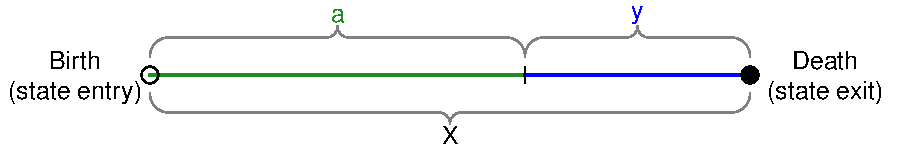
\includegraphics[scale=.8]{Figures/LifeLine.pdf}	
\end{figure}
Figure~\ref{fig:line} gives a schematic representation of this simple
relationship between age and the lifespan for a single person-life. The lived
part we call ``age'' and the yet-unlived part has no common name. Both $a$ and $y$ are placemarkers on the
lifeline and could therefore be called ``age''. We refer to these indices as
\textit{chronological} and \textit{thanatological} age, respectively.\footnote{Thanatos was the Greek god of death, which marks the end of the lifeline to which $y$ relates. By this token, one could just call chronological age \textit{aphrodesian} age, but this would probably confuse things.}
The chronological and thanatological age perspectives are applicable to state
durations in general, but in this paper we focus on the full lifespan.

For a cohort, the distribution of $X$ is given by $f(X)$, which is equal to the
lifetable death distribution, $d(a)$, for $a = X$, when the lifetable is
specified with a radix equal to unity ($l(0)=1$).
The definition of the survival-conditioned distribution of \textit{remaining}
lifetime $f(y|a)$ can be summarized in words as the probability of surviving $y$
years in the future given survival to current age $a$, and then dying at the
exact age $a+y$.\footnote{A more explicit defintion is provided in the
appendices.} Figure~\ref{fig:fya} shows selected cross-sections of the $f(y|a)$
surface calculated from the 2010 US male period lifetable \citepalias{HMD}. The area under each chronological age-conditioned curve is equal to one.
In all cases where the underlying mortality pattern is fixed, the central mass
of the curve approaches zero, moving one year down per year lived.
In these data, the shape of the center of the curve does not change much until
after chronological age 60, where conditional rescaling drives up death probabilities more and more. Upward
scaling continues beyond those ages shown here, with $y=0$ becoming the greatest
single value in all ages beyond the modal chronological age at death.

 \begin{figure}[h]
\centering
% Figure produced in R/fya.R
	\caption{Probability of surviving y years given survival to current age $a$, US
	males, 2010}
	\label{fig:fya}
	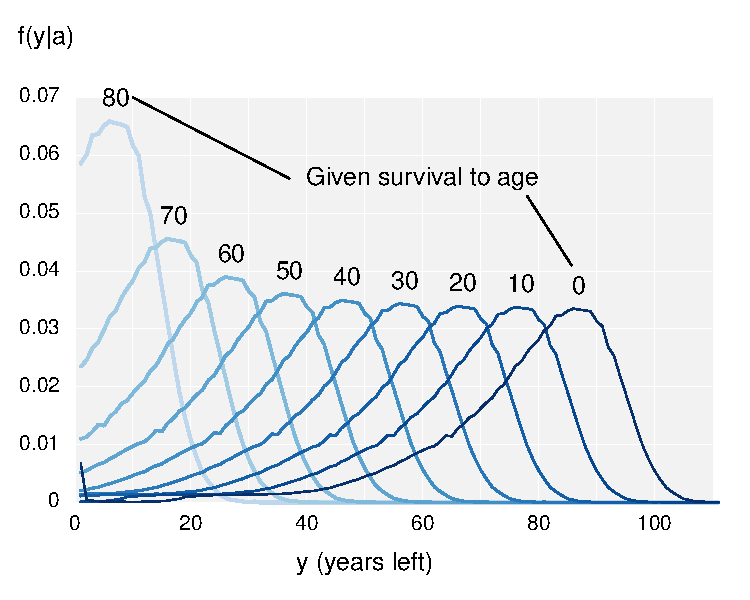
\includegraphics[scale=.8]{Figures/fya.pdf}	
\end{figure}

$f(y|a)$ can be used to calculate the population having survived to age $a$ and
with $y$ remaining years of life as $P(a,y) = P(a)f(y|a)$, where the total
population with $y$ remaining years of life, $P(y)$, is simply $\int
_{a=0}^\infty P(a,y) \dd a$ \citep{brouard1986structure, brouard1989mouvements},
a single death cohort with members from many birth cohorts. This decomposition sorts the lifeline segments of a living population
by the part yet-unlived (years left, $y$) rather than by the part lived. 
The indices $a$ and $y$ differentiate between the past and future
parts of a lifeline, respectively, and by extension of populations when
so structured. As \citet{brouard1986structure}, when comparing the lived and
to-be-lived part of a population, we refer to $P(a)$ and $P(y)$.
Is it so clear that the dead are no longer part of the population? If a life is
completely saved, this life stays in the living population and is not counted
as a death, but we (in common thinking) often imagine saved lives as a transient
state classification.
For demographers, however, among the living there
are no saved lives but only lived lives. Still we can quantify
hypothetically saveable life, and for this we must look to deaths.
It is nice, and often realistic, to think that many of the lives taken by death
are or will one day be saveable, but it is difficult to know what mortality
rates would apply to a population of saved individuals. Consider
the hypothetical population of lives saved a single time from death and subject to
the same mortality as the population at large.

Figure~\ref{fig:Day} (left) shows US 2010 period
deaths (the universe of lives that we counterfactually save) by age and sex (males on the left, females on the
right).
Over 1.23 million deaths each were recorded for US males and females in 2010. Deaths have been decomposed into discrete
categories of remaining years of life (see appendix
equation~\eqref{eq:fya}), under the assumption that saved lives are subject to
the same mortality schedule as the rest of the population and that all 2010
deaths get saved (just once). The results of this decompositon are represented
by color bands in Figure~\ref{fig:Day}. The average chronological age at death
observed for males was a full seven years lower than that for females: 69.9
versus, 76.3, respectively.\footnote{This differs from period life expectancy
(76.4 versus 81.2, respectively) because the population structure is not
stationary.}
Figure~\ref{fig:Dya} (right) displays the same decomposition after swapping the y axis and color gradient from Figure~\ref{fig:Day}. Now thanatological age (years left) of hypothetically saved lives are the primary y axis, while chronological age groups (years lived) are displayed with color. Figure~\ref{fig:Dya} communicates that most saveable lives would live short remaining lifespans once saved and granted the same lifetable mortality. This is so in this data because most saveable lives are already in chronological ages subject to high mortality rates. In general, the only saveable lives that might live very long remaining lifespans are the few deaths that occur in young ages. 

Randomly
selected saveable males from this population would have on average longer
remaining lifespans than randomly selected saveable females (16.3 versus 13.7
years, respectively). This is a paradox because females have lower mortality rates in
nearly all ages, and have longer remaining life expectancies in all ages. Female
mortality advantage is in this case more than offset by the relative youth of
male deaths. Untangling the paradox further becomes a recursive exercise,
since the relative youth of male deaths is due to an interaction between
mortality schedules and population structure, itself a result of past
vital forces.

\begin{figure}
\centering
\caption{Potentially saveable lives (deaths) in the US by sex, 2010}
\label{fig:1}
\begin{subfigure}[b]{.48\linewidth}
\centering
	\caption{Classified by age (years lived) and sex, and decomposed
by hypothetical remaining years of life (years left).}
	\label{fig:Day}
	% Figure produced in R/AllCauseFigures.R
	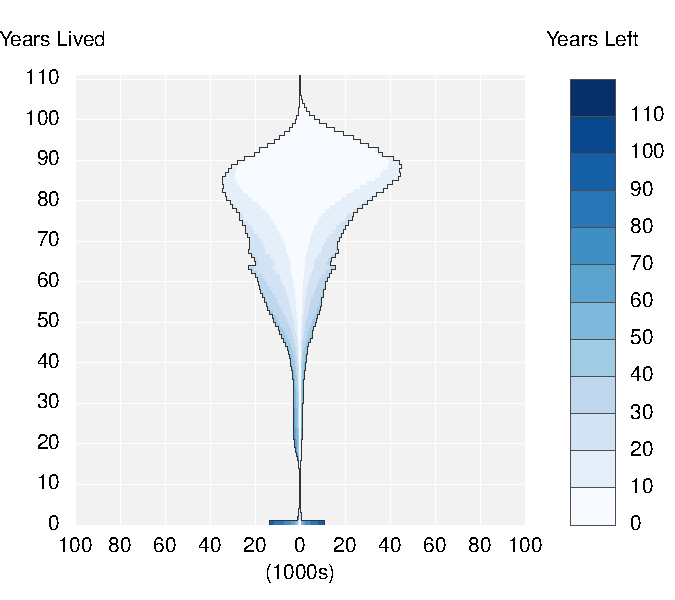
\includegraphics[scale=.55]{Figures/Deathsxy10.pdf}	
	\caption*{$D^s(a)$ from appendix equation~\eqref{eq:Dsa}}
\end{subfigure}
~
\begin{subfigure}[b]{.48\linewidth}
\centering
    \caption{Classified by hypothetical remaining years of life
(years left) and sex, and decomposed by age (years lived).}
	\label{fig:Dya}
	% Figure produced in R/AllCauseFigures.R
    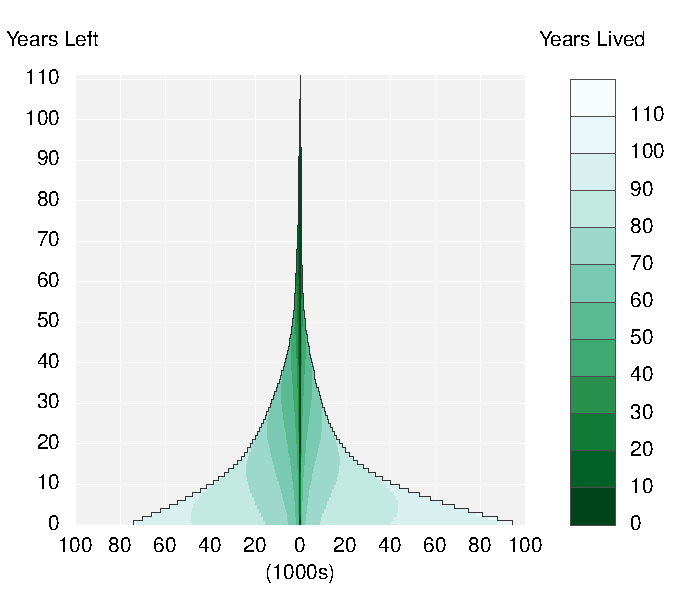
\includegraphics[scale=.55]{Figures/Deathsyx10.pdf}
    \caption*{$D^s(y)$ from appendix equation~\eqref{eq:savedy}}
\end{subfigure}
\end{figure}

\begin{figure}
\centering
\caption{Potentially person years of life won in the U.S. by sex, 2010*}
\label{fig:2}
\begin{subfigure}[b]{.48\linewidth}
\centering
	\caption{Classified by age at hypothetical saving and sex, $W^s(a)$, and
	decomposed by future ages to be lived.}
	\label{fig:SavedGained}
	% Figure produced in R/AllCauseFigures.R
	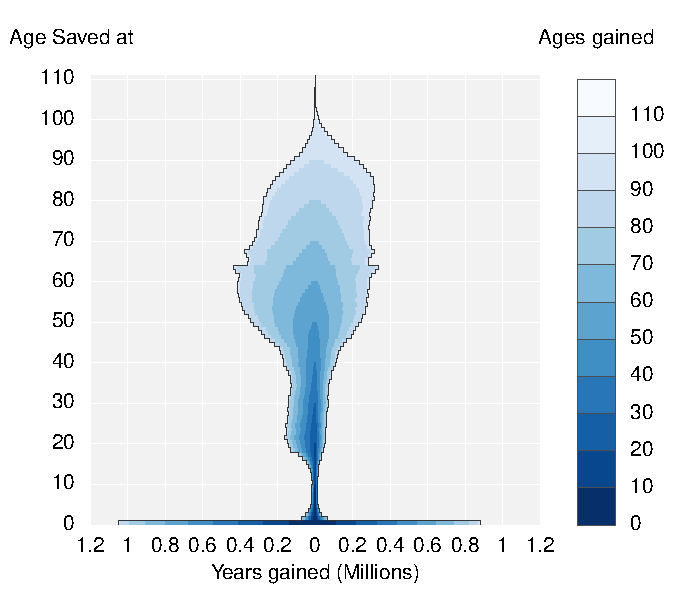
\includegraphics[scale=.55]{Figures/YearsSavedGainedxx10.pdf}
	\caption*{$W^s(a)$ from appendix equation~\ref{eq:savedea}}	
\end{subfigure}
~
\begin{subfigure}[b]{.48\linewidth}
\centering
    \caption{Classified by cumulative ages to be lived through and sex, and
    decomposed by age at saving.}
	\label{fig:LostLived}
	% Figure produced in R/AllCauseFigures.R
    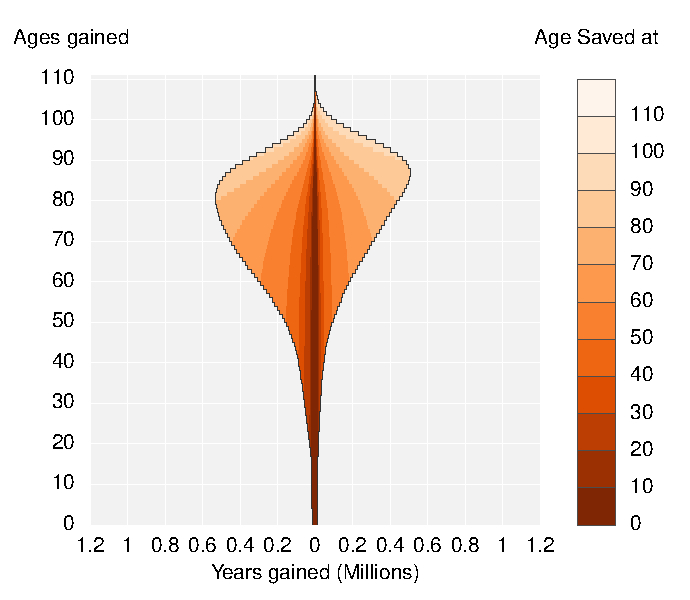
\includegraphics[scale=.55]{Figures/YearsLostLivedyx10.pdf}
    \caption*{$W^s(a+y|a)$ from appendix equation~\ref{eq:gaineday}}	
\end{subfigure}
\caption*{*Note different x scale from Figure~\ref{fig:1}.}
\end{figure}

Figure~\ref{fig:SavedGained} shows the person years of life potentially won by
saving all the deaths in each age (see appendix
equation~\eqref{eq:savedea}) for the same US data, which is essentially a
reweighting of Figure~\ref{fig:Day} by the standard age-pattern of remaining
life expectancy that these lives would hypothetically be subject to.
Color bands are assigned by decomposing the total life to be lived into the ages through which it will be lived. For example, if we save all 11700 of the 50-year-old US
males that died in 2010, they would live a total of 349000 combined years (under
a fixed 2010 mortality schedule), spread out over ages 50
and higher according to $\frac{l(50+y)}{l(50)}$. In Figure~\ref{fig:SavedGained}
we decompose these gained years of life according to the survival-conditioned
distribution of remaining lifetime (see appendix
equation~\eqref{eq:savedy}) and highlight this decomposition with color, while in Figure~\ref{fig:LostLived}, \textit{gained} ages become the primary y axis, and color bands represent the ages in which populations in each age group were saved.

Figure~\ref{fig:LostLived} represents the cumulative contribution to the
population pyramid that would result from saving all lives in 2010 and then
surviving them forward according to 2010 mortality conditions. The chronological
age axis indexes ages that are lived through at some point in the
future, in sequence rather than simultaneously. Under the same assumption of
fixed schedules, one could multiply this cumulative age structure with other
age-schedules, such as age-specific fertility rates, or the economic age profiles produced by
the NTA project, to benchmark the cumulative impacts of mortality on other
quantities of interest. For instance, the females
who died in 2010 would have given birth to 54122 babies cumulatively over their
remaining lifetime assuming they were subject to constant 2010 period fertility
\citepalias{HFD} and mortality. In the present work, we only treat age
structure, and we do not examine secondary consequences of this kind. 

\section*{Causes of death}
% AS: Extension to causes of death. This is the case you want to make. Saying,
% for instance, what if we eliminate mortality from heart disease? Or stroke? or hypertension? We 
% need to explain an story here and the draft needs to be shaped according to
% that. I think that all your mathematical material is very relevant but we need to get deeper into 
% the general idea and maybe leave the formulas for an appendix. But it is ok
% for the moment, we will think about that later.

These basic relationships carry over when deaths and survival are adjusted to
account for the hypothetical elimination of particular causes (in the case of
independence). In this case, the total number of deaths observed, $D$, is the
sum of the deaths from $n$ causes. To speak of eliminating cause $c$ (for
instance, deaths from pancreatic cancer) from the lifetable is to speak of
saving $D^{c}$ lives and then subjecting them to mortality after
having deducted cause $c$ from the lifetable.
This is problematic in that causes are not independent, and in that
reductions in cause-specific mortality are not so thorough and immediate, but it
serves as a basis for comparing the relative impacts of different causes on
a given population structure. Humans have succeeded in eradicating certain
causes of death in the past, and it
is not so audacious to imagine that we may do so yet. While these
eliminations may not deduct 100\% of their magnitude from all-cause mortality
due to substitution, there is an undeniable all-cause benefit, and at least 
we know its bounds. For some causes of death, independence is easier to imagine,
such as deaths due to needless violence or particular kinds of accidents. We
demonstrate concepts using large cause groupings.

\vspace{2em}
% latex table generated in R 3.0.1 by xtable 1.7-4 package
% Tue Mar 31 12:34:12 2015
% added column titles by hand\ldots
\begin{minipage}{\linewidth}
\centering
\captionof{table}{Major causes of death in the U.S. by sex, 2010 (HMD)}
\label{tab:counts}
\begin{tabular}{rrrrrrr}
\hline
Cause &\multicolumn{2}{c}{ Female }&\multicolumn{2}{c}{ Male
}&\multicolumn{2}{c}{ Total}
\\
 & count & \% & count & \% & count & \% \\ 
  \hline
   Cardiovascular & 395200 & 32.0 & 383077 & 31.1 & 778277 & 31.5 \\ 
Cancer* & 369411 & 29.9 & 366373 & 29.7 & 735785 & 29.8 \\ 
  Infectious & 156086 & 12.6 & 149139 & 12.1 & 305226 & 12.4 \\ 
  External & 60673 & 4.9 & 125733 & 10.2 & 186405 & 7.6 \\ 
    Mental & 76270 & 6.2 & 41413 & 3.4 & 117683 & 4.8 \\ 
  Infant* & 10368 & 0.8 & 12119 & 1.0 & 22487 & 0.9 \\ 
  Other & 167995 & 13.6 & 154577 & 12.5 & 322572 & 13.1 \\ 
  \hline
  Total & 1236003 & 100.0 & 1232432 & 100.0 & 2468435 & 100.0 \\
   \hline
\end{tabular}\par
\raggedright\small
*The ``cancer'' group includes diseases of the nervous
system. The ``infant'' category includes all congenital conditions, including
those that result in death after infancy. 
\end{minipage}
\vspace{2em}

Table~\ref{tab:counts} lists a selection of grouped causes of death for the
United States in 2010. The cardiovasclar category listed here combines
various diseases of the heart, blood, and circulatory system. Cardiovascular
diseases are the largest killer of both males and females, followed closely by
the broad cancer category. Together, these two categories, which include most
degenerative diseases, accounted for over 60\% of deaths in the United States in
2010. For the following illustrations, we focus on cardiovascular
diseases.

Now Figures~\ref{fig:1} and~\ref{fig:2}
can be repeated for any particular cause of death, and the profile of each of the four perspectives
characterizes the population impact of the given cause of death.
Figures~\ref{fig:5} and~ \ref{fig:6} depict the same temporal viewpoints,
respectively, but now the deaths decomposed are only deaths to cardiovascular
causes, and cardiovascular causes have been eliminated from the lifetable functions used for decomposition and
 redistribution. Causes differ in their impact profiles, and this forms a
 basis for comparison. As with standard population pyramids, one may prefer the
 use of percent scales to facilitate comparisons between causes or countries. These
 figures for cardiovascular causes give visual form to the intuition that demographers
 have about cardiovascular causes of death. Cardiovascular causes are important in
 older ages, and kill similar numbers of males and females. Saving a randomly
 selected death from a cardiovascular cause will on average have a slightly
 lower payoff in terms of expected years of life gained than does preventing a death in general. Further, a typical life saved will traverse many working ages, and reach well into old
 ages.
 The age groups with the most to gain by eliminating external causes are males
between ages 55 and 65 and females in their 80s (clearest in
Figure~\ref{fig:6}).
 
 The average chronological age of deaths to cardiovascular causes in the USA in
 2010 was 74.4 for males and 81.8 for females. Their cause-deleted mean
 remaining lifetimes would have been 16.0 and 13.0 years,
 respectively. This version of mean remaining lifetime refers to
 observed deaths, as depicted in Figure~\ref{fig:Dyac}, not the stationary
 lifetable measures. The same means from the stationary population would be 12.5
 and 10.9, for males and females, respectively, and these latter figures can
 be treated as hypothetical expectancies. The mean
 age-at-saving of all the person-years hypothetically won under these same conditions becomes 65.1 for males and 72.4 for females, whereas the mean of the ages \textit{enjoyed} by these hypothetically saved people are 78.0 and 83.7,
 respectively. 
 
\begin{figure}
\centering
\caption{Deaths from cardiovascular causes in the USA, 2010}
\label{fig:5}
\begin{subfigure}[b]{.48\linewidth}
\centering
	\caption{Classified by age (years lived) and sex, and decomposed
by hypothetical remaining years of life (years left).}
	\label{fig:Dayc}
	% Figure produced in R/SingleCauseExampleFigures.R
	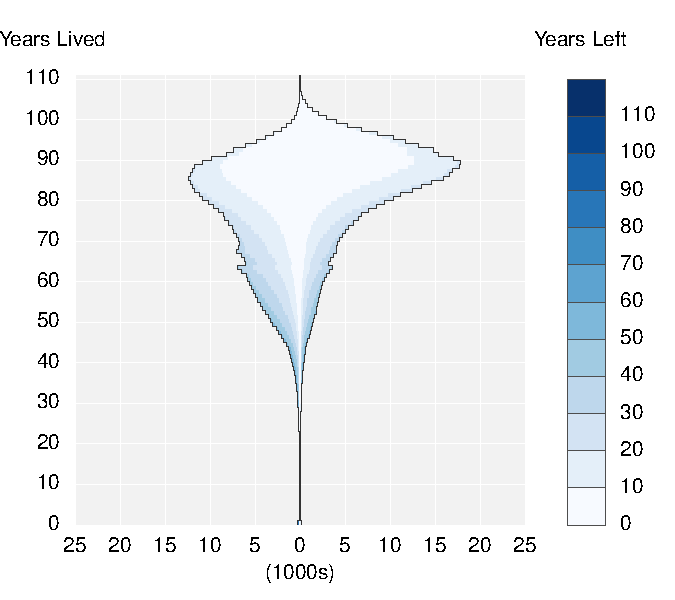
\includegraphics[scale=.55]{Figures/Deathsxy10USACardio.pdf}	
	\caption*{$D^{s~cardio}(a)$}
\end{subfigure}
~
\begin{subfigure}[b]{.48\linewidth}
\centering
    \caption{Classified by hypothetical remaining years of life
(years left) and sex, and decomposed by age (years lived).}
	\label{fig:Dyac}
	% Figure produced in R/SingleCauseExampleFigures.R
    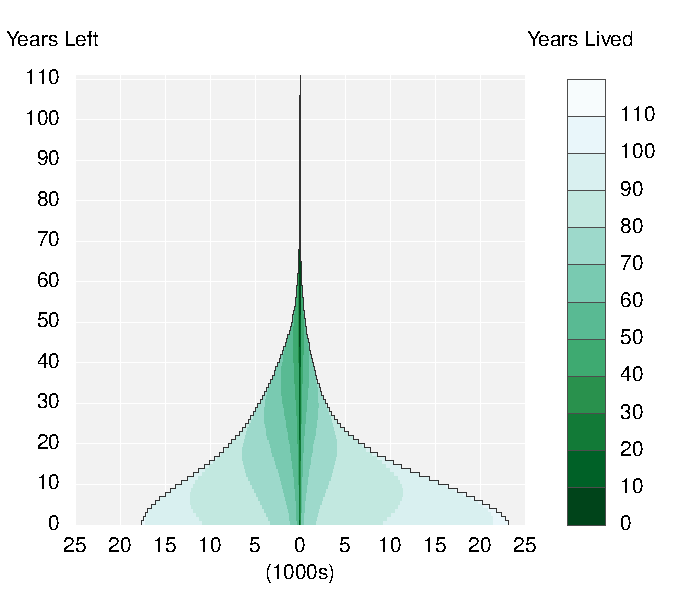
\includegraphics[scale=.55]{Figures/Deathsyx10USACardio.pdf}
    \caption*{$D^{s~cardio}(y)$ }
\end{subfigure}
\end{figure}


\begin{figure}
\centering
\caption{USA, 2010 Deaths from cardiovascular causes, years of life potentially
won*}
\label{fig:6}
\begin{subfigure}[b]{.48\linewidth}
\centering
	\caption{Classified by age at hypothetical saving and sex, $W^s(a)$, and
	decomposed by future ages to be lived.}
	\label{fig:SavedGainedUSACardio}
	% Figure produced in R/SingleCauseExampleFigures.R
	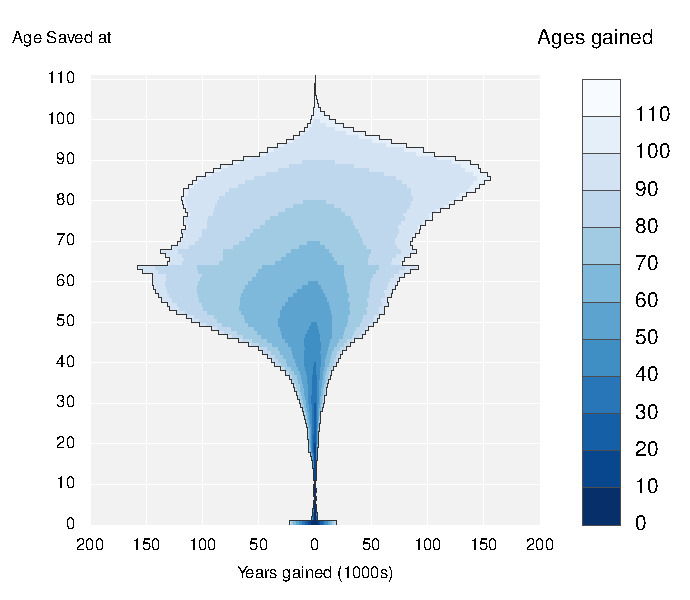
\includegraphics[scale=.55]{Figures/YearsSavedGainedxx10USACardio.pdf}
	\caption*{$W^{s~cardio}(a)$ from appendix equation~\ref{eq:savedea}}	
\end{subfigure}
~
\begin{subfigure}[b]{.48\linewidth}
\centering
    \caption{Classified by cumulative ages to be lived through and sex, and
    decomposed by age at saving.}
	\label{fig:LostLivedUSAExternal}
	% Figure produced in R/SingleCauseExampleFigures.R
    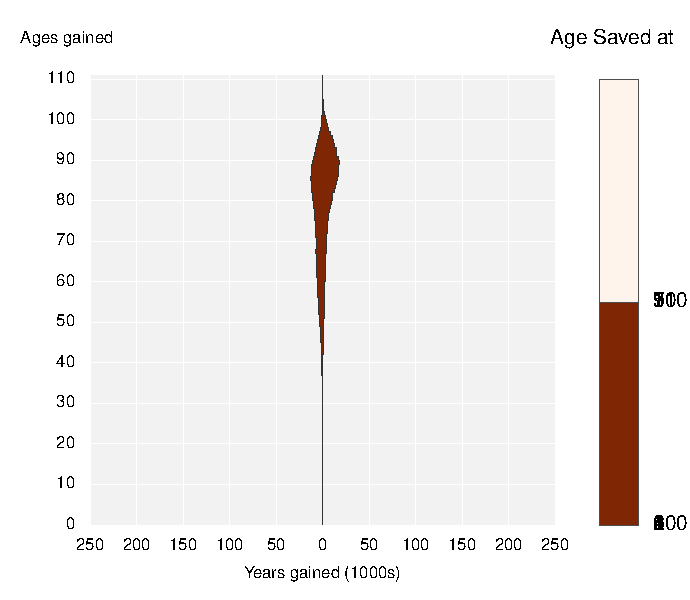
\includegraphics[scale=.55]{Figures/YearsLostLivedyx10USACardio.pdf}
    \caption*{$W^{s~car}(a+y|a)$ from appendix equation~\ref{eq:gaineday}}	
\end{subfigure}
\caption*{*Note different x scale from Figure~\ref{fig:5}.}
\end{figure}

\FloatBarrier

 Means do not tell the story as well as images, but they allow for easy
 comparisons. Table~\ref{tab:obssummary} gives a summary of the same measures
 for males and females for each of the seven causes of death listed in
 Table~\ref{tab:counts}, where $\bar{a}^c$ is the observed mean chronological
 age at death for cause $c$, $\bar{y}^c$ is the mean thanatological age for
 cause $c$ were all deaths of this cause to be saved, $\widebar{W(a)}^c$ is mean
 age-at-saving of all of the person years of life that would be gained by saving
 all deaths of cause $c$, and $\widebar{W(a+y|a)}^c$ is the mean age
 lived-through after saving, under these same assumptions. From
 Table~\ref{tab:obssummary}, we learn that immediate elimination of infant and
 genital causes of death would tend to produce individuals with long lives, and
 we intuit that most of the remaining lifespan won would be lived through
 working ages. External causes are also relatively ``youthful'' in that they
 occur in you chronological ages, and preventing an external death in 2010 (and
 thereafter) would have implied on average three decades of remaining life, with
 most years of life won being centered on chronological ages that nowadays are
 considered active.
 
 \vspace{2em}
\centerline{ 
\begin{minipage}{\linewidth}
\centering
\captionof{table}{Summary of four time perspectives for the U.S. by sex, 2010
(HMD)}
\label{tab:obssummary}
% latex table generated in R 3.0.1 by xtable 1.7-4 package
% Wed Apr  1 16:34:03 2015
\centering
\begin{tabular}{rrrrrrrrr}
\hline
Cause &\multicolumn{2}{c}{ $\bar{a}^c$ }&\multicolumn{2}{c}{ $\bar{y}^c$
}&\multicolumn{2}{c}{ $\widebar{W(a)}^c$}&\multicolumn{2}{c}{
$\widebar{W(a+y|a)}^c$}\\
 & \myalign{c}{Male} & \myalign{c}{Female} & \myalign{c}{Male} & \myalign{c}{Female} & \myalign{c}{Male} & \myalign{c}{Female} & \myalign{c}{Male} & \myalign{c}{Female} \\ 
  \hline
  Cardiovascular & 74.4 & 81.8 & 16.0 & 13.0 & 65.1 & 72.4 & 78.0 & 83.7 \\ 
  Cancer* & 72.3 & 74.7 & 16.4 & 16.7 & 63.6 & 64.6 & 76.4 & 78.0 \\ 
  Infectious & 74.2 & 77.9 & 14.1 & 13.4 & 62.5 & 66.4 & 75.2 & 78.6 \\ 
  External & 47.9 & 57.1 & 34.0 & 29.8 & 36.7 & 40.3 & 59.7 & 63.3 \\ 
  Mental & 80.0 & 87.2 & 10.2 & 7.5 & 67.7 & 79.5 & 78.2 & 86.8 \\ 
  Infant* & 9.2 & 10.7 & 68.4 & 71.7 & 3.7 & 4.0 & 41.6 & 43.7 \\ 
  Other & 69.3 & 75.9 & 17.5 & 15.3 & 55.5 & 60.2 & 71.0 & 75.2 \\ 
   \hline
   All & 69.9 & 76.9 & 16.3 & 13.7 & 54.4 & 60.8 & 69.9 & 75.0 \\ 
   \hline
\end{tabular}
\raggedright\small
*The ``cancer'' group includes diseases of the nervous
system. The ``infant'' category includes all congenital conditions, including
those that result in death after infancy. 
\end{minipage}}


\section*{Discussion}

There are many perspectives under which demography can account for the
relationships between stocks and flows, but not all form part of the collective
practice of demography. 
Our objective in these exercises has been to offer a novel quantitative and
visual basis to assess the impact of mortality on population stocks.
This is done by calculating the lifespan distributions foregone due to death and indexing the results based on various aspects of the lifespan. Practical suggestions have included both chronological and thanatological age
perspectives, as well as two ways of accounting for years of lifespan gained:
(i) The years would be won by saving the deaths in age $a$, and (ii) the
ages saved individuals would pass through if survived forward.

The reader may choose to interpret this exercise as we
have narrated it: ``what would have happened if these lives had been saved?''. We wish to point out that believing
this statement is not necessary in order for the measures to be useful, just as common uses of
period life expectancy require a certain degree of suspended disbelief. For
clarity, we list the most important assumptions to be aware of when treating
data as we have.
\begin{enumerate}
\item Unchanging period rate schedules. Note that the same formulas apply when
data in the cohort perspective are used, but some care must be taken to allocate past deaths according to observed mortality within the cohort, and then complete non-extinct
cohorts' mortality experience according to
projection. \citet{brouard1986structure} combined history and projection
in this way in his original study of population structure.  In any case, period measures are the best barometer of the
present that we have, and all calculations done in this paper fall under the
period umbrella. The researcher is not limited to the use of static age
schedules, and $f(y|a)$ could be calculated for age schedules that vary
by birth cohort.
\item Homogenous populations. In using rate schedules derived from the
population at large in order to describe a hypothetical population of saved
individuals, we may neglect that saved individuals may be a frailer than the
general population, and so subject to higher mortality rates going forward. We
offer to remedy for this shortcoming, except to note that this possibility may
hold truer for some causes than for others, and in general the degree of bias is
unknown.
\item Independence of causes. As discussed in the text, all causes of death
compete to be first, and removing the first cause may not reduce the all cause
rate by the same amount we have partitioned, $\mu^c$. The final reduction will
lie somewhere between 0 and $\mu^c$, and may depend on the cause and
overall level of mortality. We think that this possible unsolvable limitation
ought not keep the researcher from exploring in this direction. With respect to
survival after lifesaving, the researcher may choose to delete the cause in
question or not. In practice, this choice makes little difference even for
large causes, due to the constraints of lifetable entropy.
\end{enumerate}



%Then, decide whether to present a separate panel for each country of all causes
%for each perspective, or rather each cause in a unique panel comparing
%countries. I'm leaning toward each each country in a separate panel, but need
% to think on it more. I'm doubting whether it makes sense to compare populations
%that are not stable, since part of differences will be due to previous
%population structure. Comparing causes (save for competing risks) works within
% a population because it has a single structure, but between countries it may only
%make sense to go back to rates, but then we lose the point of the paper. This
% is my tentative stance on between-country comparisons. It's of course all easy to
%decompose, but that seems like a frivolous step.
% AS: Regarding expanding the analysis to more populations, I think that you are
% right, but part of the differences would be not only due to the structure but the context 
% of each population.
% 
---------------------------------------
\bibliographystyle{plainnat}
  \bibliography{references}  


\begin{appendices}
\section{Formulas}
The probability of surviving exactly $y$ years into the future given survial to
age $a$, $f(y|a)$ is given by:\footnote{This definition is identical to
that used in \citet{brouard1989mouvements}, \citet{vaupel2009life} or
\citet{rao2014generalization} in proving the equality of chronological and
thanatological age structure in stationary populations. Brouard apparently had
proven this earlier than 1989, since he cites the relationship in
\citet{brouard1986structure}. Equation \eqref{eq:fya} is easily modifiable to
account for mortality schedules that change over time.}
\begin{equation}
\label{eq:fya}
f(y|a) = \mu(a+y) \frac{l(a+y)}{l(a)} \tc
\end{equation}
where $\mu(a)$ is the force of mortality at exact age $a$, and $l(a)$ is
the value of the survival function at exact age $a$, proportional to the
probability of surviving from birth to age $a$. 


Assume that all the deaths recorded in a year are saved and brought back to
life. One may ask much more than the number and age structure of these saved
lives, $D^s(a)$,
\begin{equation}
\label{eq:Dsa}
D^s(a) = \mu(a)P(a) \tc
\end{equation}
but also how many years the people saved at age $a$ would live, 
$W^s(a)$\footnote{A mnemonic for $W$ could be \textit{won} years. This is
essentially an age at death breakdown of YPLL.}? The simplest calculation is
to multiply the number of gained survivors by remaining life expectancy at each
age, $e(a)$:
\begin{align}
\label{eq:savedea}
W^s(a) = D^s(a)e(a) &= P(a)\mu(a)\frac{1}{l(a)}\int l(a+y) \dd y \tp
%\notag\\
         %&= \mu(a)\int_{y=0}^\infty B(t-a)l(a+y) \dd y 
\end{align}
$D^s(a)e(a)$ classifies potentially saved person-years by the
ages in which they were saved. One may also wish to know the distribution of remaining lifespans of saved
lives, which is quite different from \eqref{eq:savedea}:
\begin{equation}
\label{eq:savedya}
D^s(a)f(y|a) = P(a)\mu(a)\mu(a+y) \frac{l(a+y)}{l(a)} \tp
\end{equation}
Equation \eqref{eq:savedya} aggregates up to the thanatological age distribution
of saved lives, $D^s(y)$:
\begin{equation}
\label{eq:savedy}
D^s(y) = \int D^s(a)f(y|a) \dd a \tp
\end{equation}
%or the time-to-death distribution of the total years of life
%gained,
%\begin{equation}
%\label{eq:gainedy}
%W^s(y) = \int D^s(a)\frac{l(a+y)}{l(a)} \dd a \tc
%\end{equation}
Or one might ask through which chronological ages the gained years of life
would be lived, $W^s(a+y|a)$,
\begin{equation}
\label{eq:gaineday}
W^s(a+y|a) = D^s(a)\frac{l(a+y)}{l(a)} \tp
\end{equation}

Define the force of mortality, $\mu(a) = \sum _{c=1}^n \mu^c(a)$,
as the sum of $n$ categorically separable causes. The people that will die from
cause $c$ are:
\begin{align}
D^c &= \int_0^\infty D^c(a) \dd a \\
&= \int_0^\infty \mu^c(a)P(a) \dd a \tc\\
\intertext{and to hypothetically save all these people is to remove cause $c$
from mortality, retaining $D^c$ lives in the population. It makes sense to
calculate the distribution of remaining lifespans of the $D^c$ people that would
have died of this cause using $l(a)$ removed of the cause in question, so we define
$l^{-c}(a)$,}
l^{-c}(a) &= e^{-\int _0^a \mu(a)-\mu^c(a) \dd a} \tc\\
\intertext{which is hopefully more legible to render as}
l^{-c}(a) &= e^{-\int _0^a \mu^{-c}(a) \dd a} \tp\\
\intertext{This is a stronger supposition than the idea of repeated
resuscitation from \citet{vaupel1987repeated}, but the idea is to separate out
the impacts of particular causes.
Let us continue with the same notational concept of ${ }^{-c}$ to define
remaining life expectancy assuming survival to age $a$ and no more death from cause $c$ after age $a$, $e^{-c}(a)$:} e^{-c}(a) &= \frac{1}{l^{-c}(a)}\int _{y=0}^\infty l^{-c}(a+y) \dd y \tp
\end{align}
and so on, repeating equations \eqref{eq:savedea} and \eqref{eq:savedy} for the
case of cause-specific saveable lives and their cause-deleted remaining
lifespans.

In these equations, all quantities are derived on the basis of a mortality
schedule and a given population structure, $P(a)$. Note that $P(a)$
can also be defined as the stationary population structure implied by the given
mortality conditions. In this case the interpretations are essentially the same,
but impacts on population structure derived in this case would refer to a
theoretical population that itself is completely a function of mortality.
Summary results comparable to those given in the main text are reproduced in an
appendix for the case of a stationary population.

\section{Stationary-equivalent summary results}

Table~\ref{tab:atatsummary} provides the same mean statistics as table
\ref{tab:obssummary}, except that now instead of calculating on the basis of the
mortality and population of the United States in 2010 we use the 2010 mortality
conditions in conjunction with the stationary population they imply. These means
have the same interpretation as those presented in the text, except that they
are relevant for the theoretical stationary population, and are
therefore entirely the product of the vital force of mortality. All results are
therefore different than those relevant for the case of 2010, but not
remarkably so, because the 2010 US population structure was
coincidentally close to stationary. The cause of death that is most similar
between the stationary and observed populations is infant and congenital
conditions. This cause is highly concentrated in age 0 and youth, which means
that thanatological redistributions of this cause approximate redistributing a
lifetable radix, pulling patterns close to the stationary state. Other causes
and measures differ by as much as \%35 in this case between the observed and
stationary populations. We report observed patterns in the main text because
these are of more immediate relevance.


\vspace{2em}
\centerline{ 
\begin{minipage}{\linewidth}
\centering
\captionof{table}{Summary of four time perspectives for the U.S. 2010 stationary
population by sex, 2010 (HMD)}
\label{tab:atatsummary}
% latex table generated in R 3.0.1 by xtable 1.7-4 package
% Wed Apr  1 16:34:03 2015
\centering
\begin{tabular}{rrrrrrrrr}
Cause &\multicolumn{2}{c}{ $\bar{a}^c$ }&\multicolumn{2}{c}{ $\bar{y}^c$
}&\multicolumn{2}{c}{ $\widebar{W(a)}^c$}&\multicolumn{2}{c}{
$\widebar{W(a+y|a)}^c$}\\
 & \myalign{c}{Male} & \myalign{c}{Female} & \myalign{c}{Male} & \myalign{c}{Female} & \myalign{c}{Male} & \myalign{c}{Female} & \myalign{c}{Male} & \myalign{c}{Female} \\ 
  \hline
  Cardiovascular & 79.8 & 85.0 & 12.5 & 10.9 & 70.9 & 77.0 & 81.7 & 86.6 \\ 
  Cancer* & 76.8 & 78.5 & 13.3 & 13.9 & 68.2 & 68.8 & 79.2 & 80.4 \\ 
  Infectious & 79.2 & 81.3 & 11.0 & 11.1 & 68.4 & 71.0 & 78.9 & 81.4 \\ 
  External & 54.9 & 64.8 & 28.9 & 24.0 & 38.8 & 43.2 & 61.0 & 65.0 \\ 
   Mental & 84.9 & 89.2 & 7.6 & 6.5 & 75.0 & 83.2 & 83.0 & 89.3 \\ 
  Infant* & 11.3 & 13.0 & 66.7 & 69.7 & 3.8 & 4.1 & 41.7 & 43.8 \\
  Other & 75.9 & 80.5 & 13.3 & 12.1 & 61.4 & 65.9 & 74.6 & 78.6 \\ 
   \hline
   All & 76.4 & 81.2 & 12.2 & 10.9 & 60.8 & 66.5 & 73.9 & 78.5 \\ 
   \hline
\end{tabular}
\raggedright\small
*The ``cancer'' group includes diseases of the nervous
system. The ``infant'' category includes all congenital conditions, including
those that result in death after infancy. 
\end{minipage}
}

Note that in the stationary population the mean age at death for all-cause
mortality is equal to life expectancy at birth, shown in this table as 76.4 and
81.2 for males and females, respectively. These figures are slightly off from
the Human Mortality Database estimates of 76.60 and 81.37, respectively, because
we have used simplified lifetable assumptions, such as assuming $L_x$ is the
linear average of $l_x$ and $l_{x+1}$, even for age zero. Further, we have not
smoothed older ages, as does the HMD. The majority of the difference in these
two figures is due to our not having given special treatment to $a_0$, the mean age
of infant deaths. This error is a small artifact, and it is more trivial for
causes of death that tend to concentrate in older ages. Further details can be
found by examining the R code provided in an online repository for this
work.\footnote{See \url{https://github.com/timriffe/YearsLost}}

%\section{Country comparison figures}
%Note to A{\"i}da:
%This is a temporary appendix, and all figures are provisional at this time. We
%just need to figure out how best to present information. For the time being we
%have six populations, and this will remain the case through PAA, it appears.
%I have taken figures \ref{fig:3} and \ref{fig:4} repeated these for each cause
%that made sense, and all sex countries, denoted with three letter codes at the
%moment. Some causes only hit one age, such as infant and
%congenital conditions (actually these appear later in life too, but in small numbers). $W(a)$ is not very useful to plot for this
%cause of death, since it is all concentrated in age 0. All x axes are now
%percent, in order to make populations of different size comparable. This works
%for each cause/perspective, but most causes have such different profiles that
%the x axes \textit{between} causes must have different ranges. So, each bundle
%of six figures is comparable within itself, but they are not comparable between
%each other. Also, note, I've been hasty and have not labeled the y axes. These
%are as in the respective figures from the text. Please just take a look for the
%time being and we can decide how best to organize things. I'll put each of the
%four figure types into appendix subsections. Each subsection will contain a
%figure for each cause that I worked with. These include cancer, cardio,
%external, ill defined, inf/cong, infectious, mental, and other (these are the
%short names for the categories I aggregated).
%\textit{Other} and \textit{ill defined} are admittedly not so interesting
%substantively, and we may as well omit them from the paper. It may make the
%most sense to just highlight a few interesting causes. Some causes/perspectives
%are very similar between countries, and some show more variety. Let's work on
%narrowing this down somehow and then decide how best to describe and display in
%the paper. 
%
%\pagebreak
%\subsection{$D^s(a)$, decomposed as in Figure~\ref{fig:Dayc}}
%Note, Infant and congenital conditions is omitted from this perspective. It
%still interesting, but better shown with a table than with a pyramid display.
%\begin{figure}
%\centering
%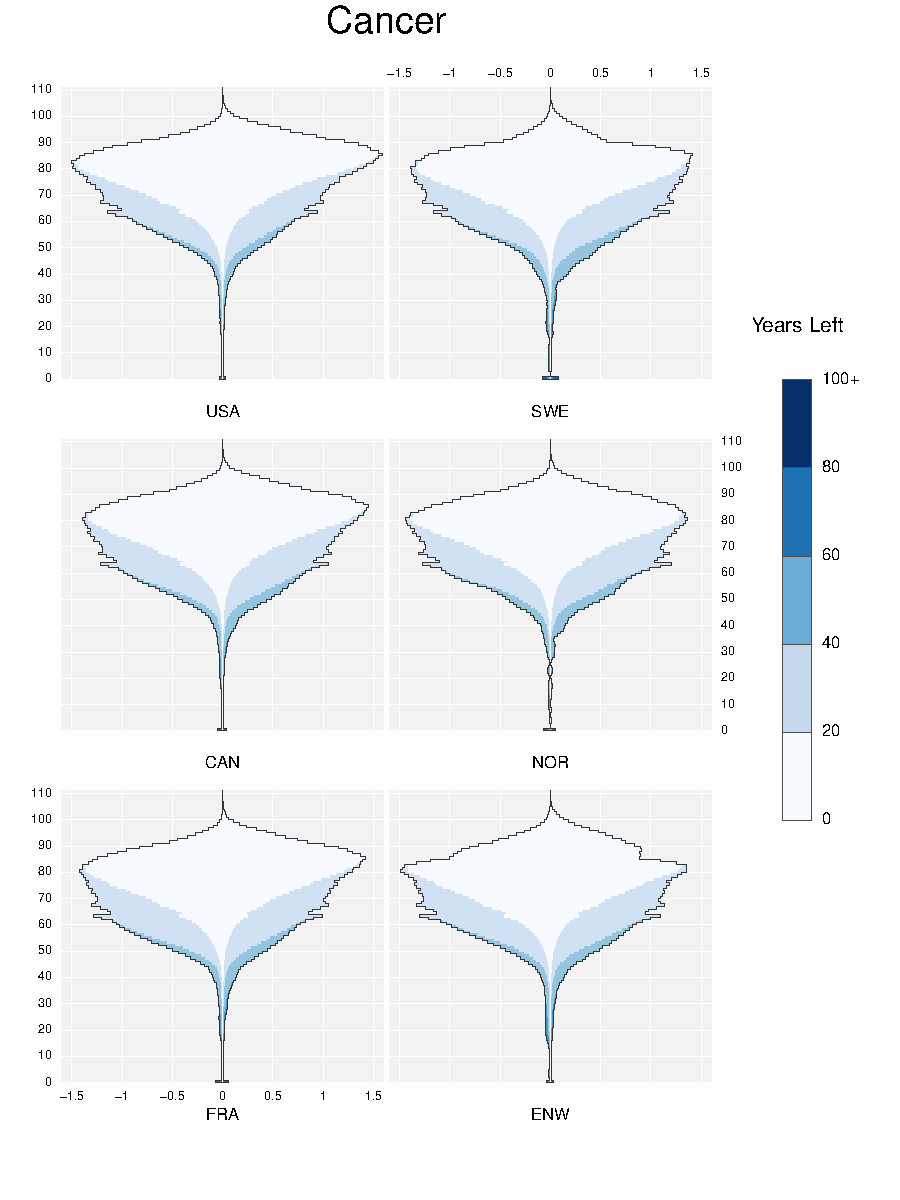
\includegraphics[scale=.8]{Figures/Causes/DxyCancer.pdf}
%\end{figure}
%\begin{figure}
%\centering
%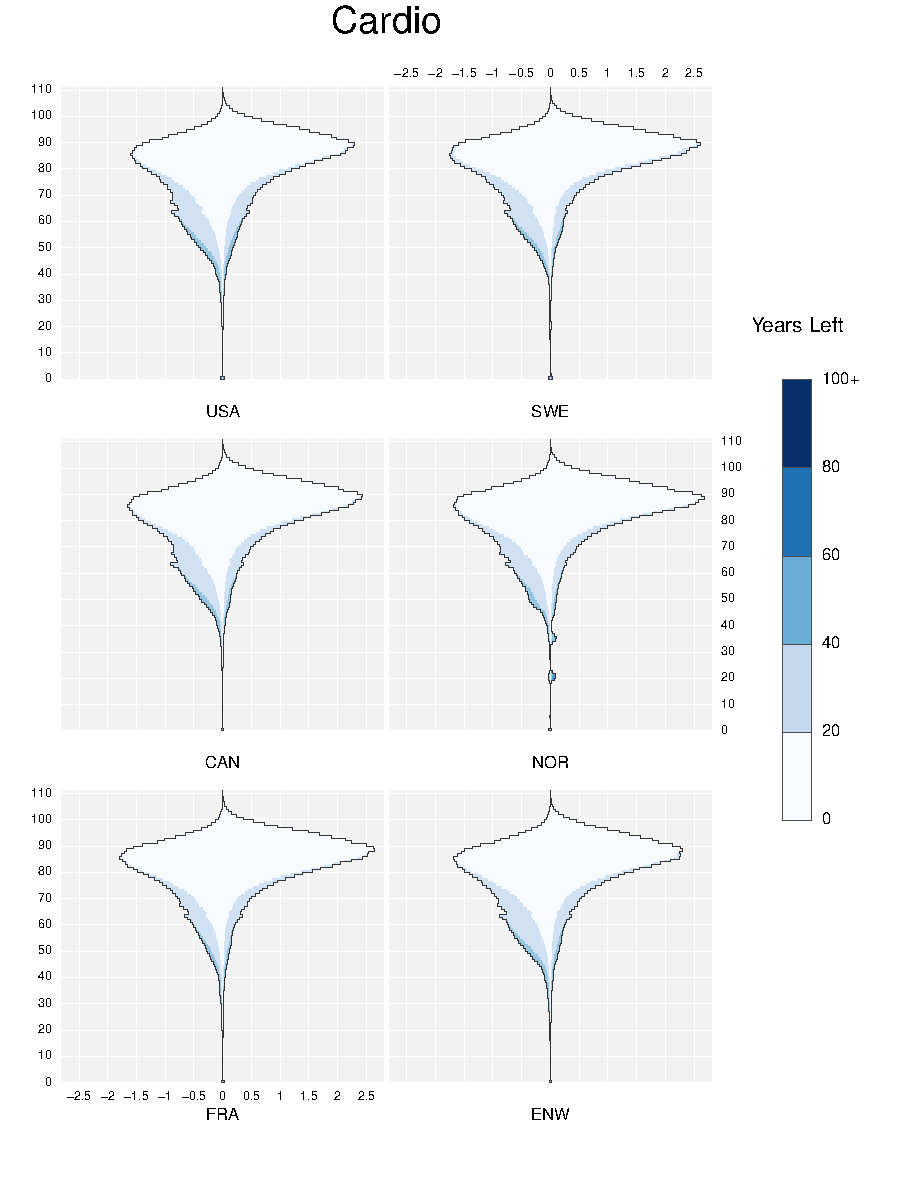
\includegraphics[scale=.8]{Figures/Causes/DxyCardio.pdf}
%\end{figure}
%\begin{figure}
%\centering
%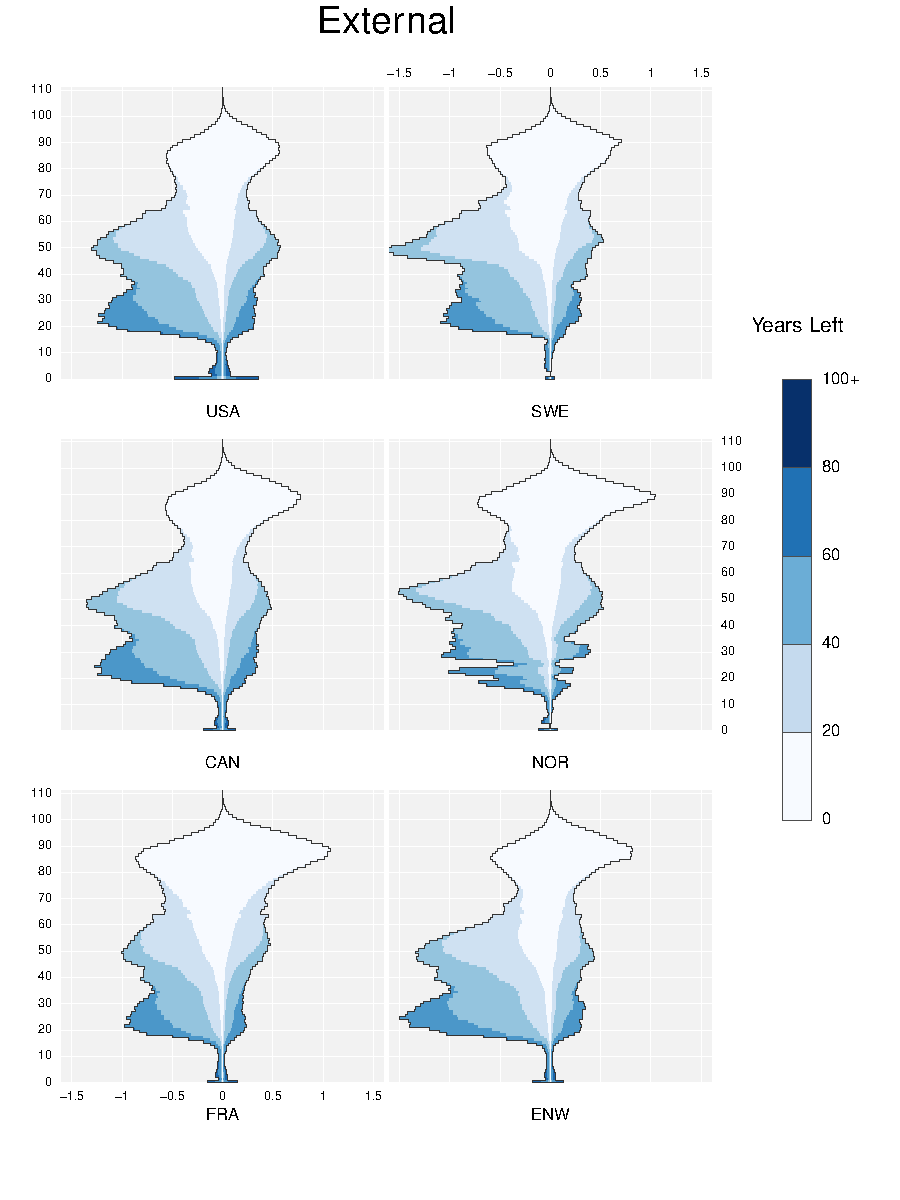
\includegraphics[scale=.8]{Figures/Causes/DxyExternal.pdf}
%\end{figure}
%\begin{figure}
%\centering
%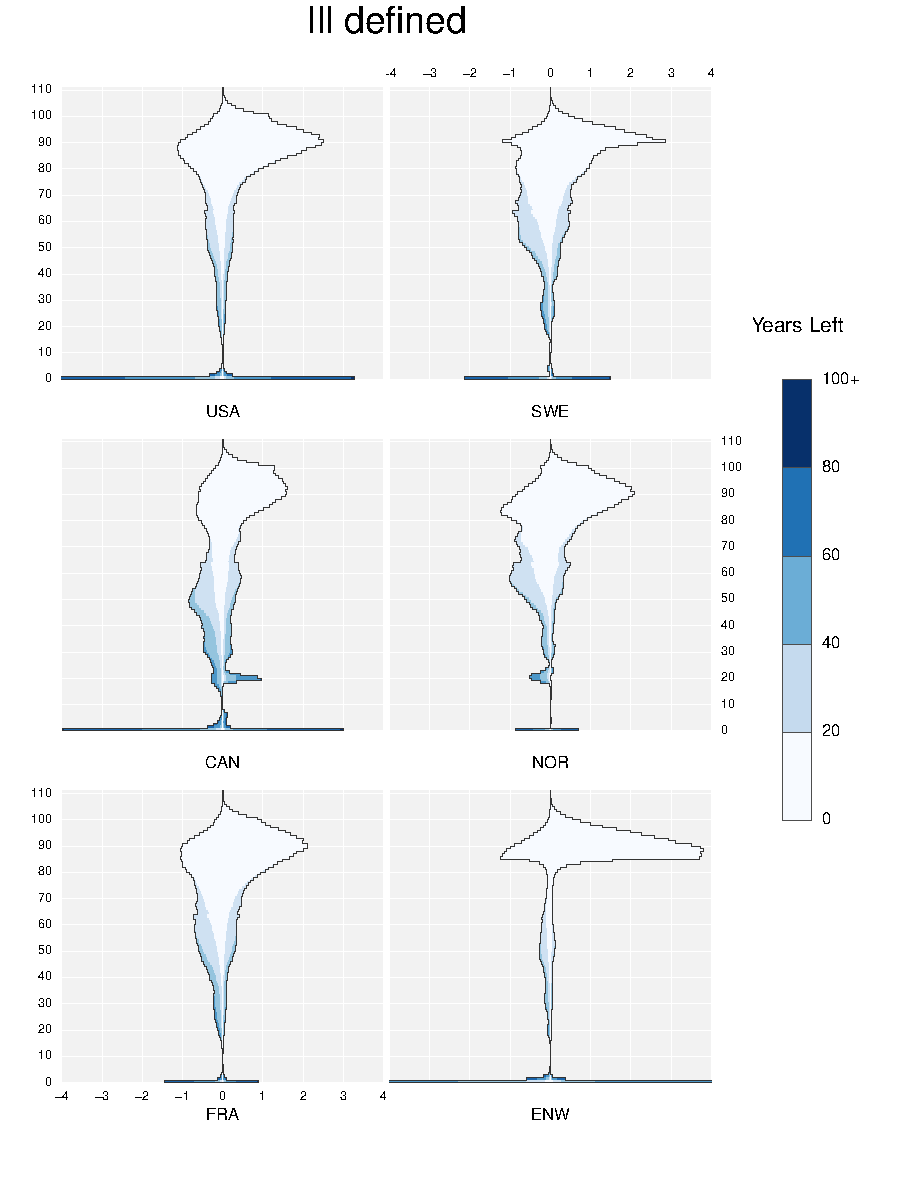
\includegraphics[scale=.8]{Figures/Causes/DxyIll defined.pdf}
%\end{figure}
%\begin{figure}
%\centering
%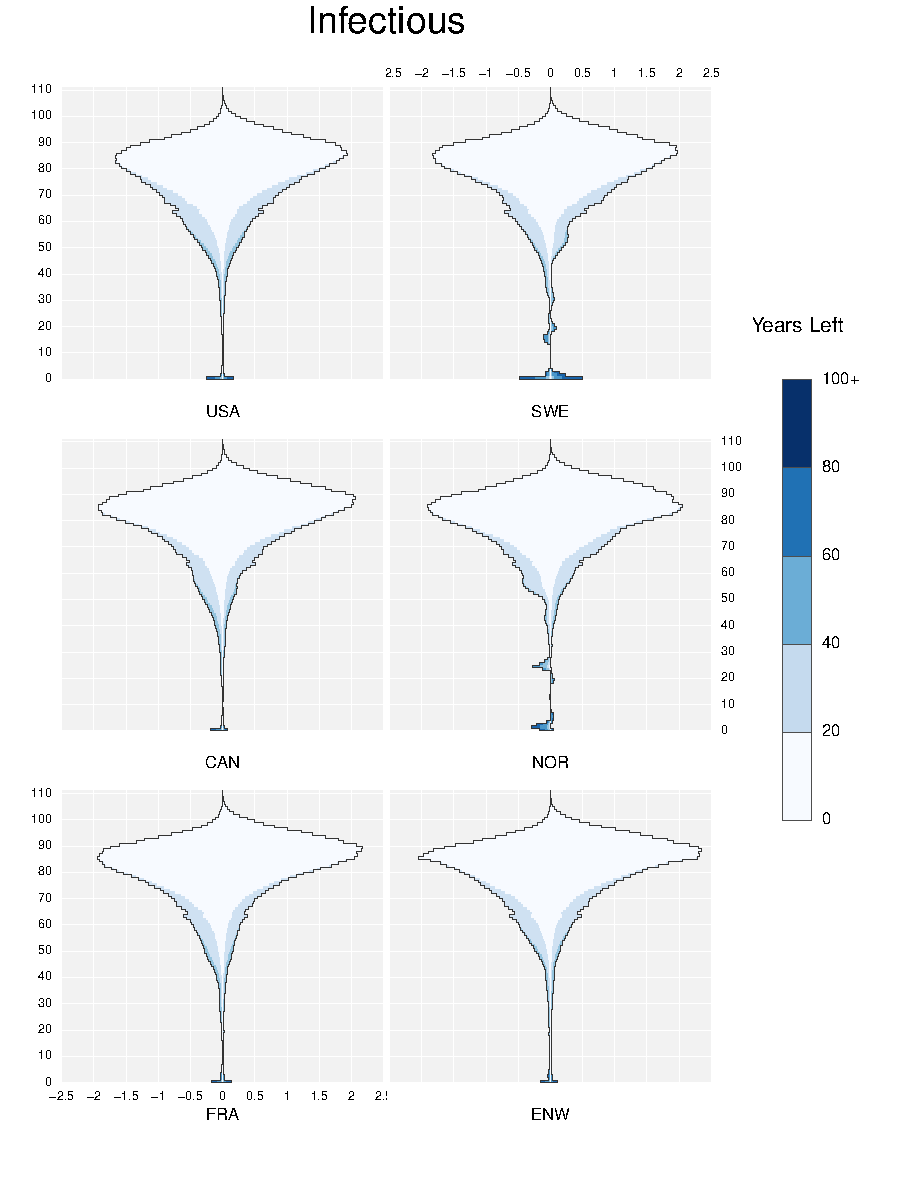
\includegraphics[scale=.8]{Figures/Causes/DxyInfectious.pdf}
%\end{figure}
%\begin{figure}
%\centering
%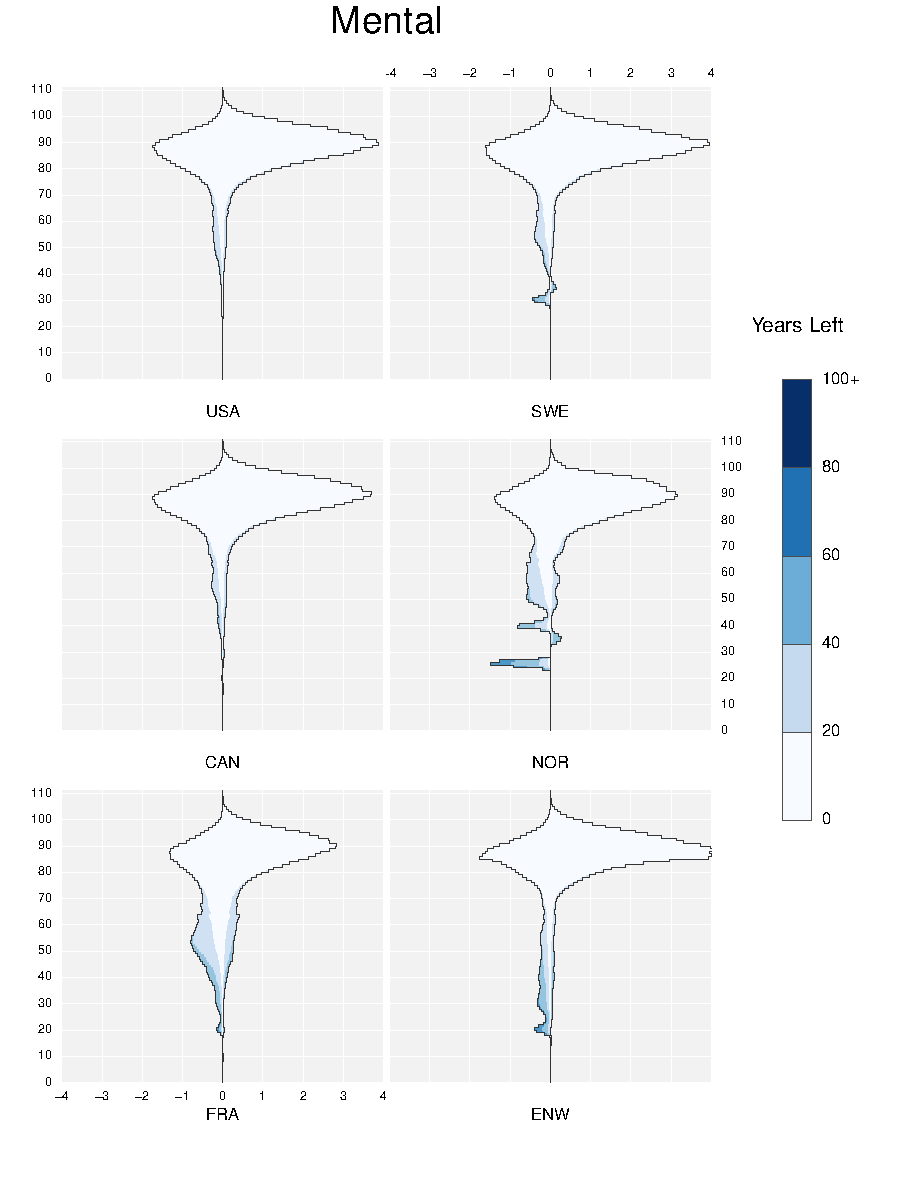
\includegraphics[scale=.8]{Figures/Causes/DxyMental.pdf}
%\end{figure}
%\begin{figure}
%\centering
%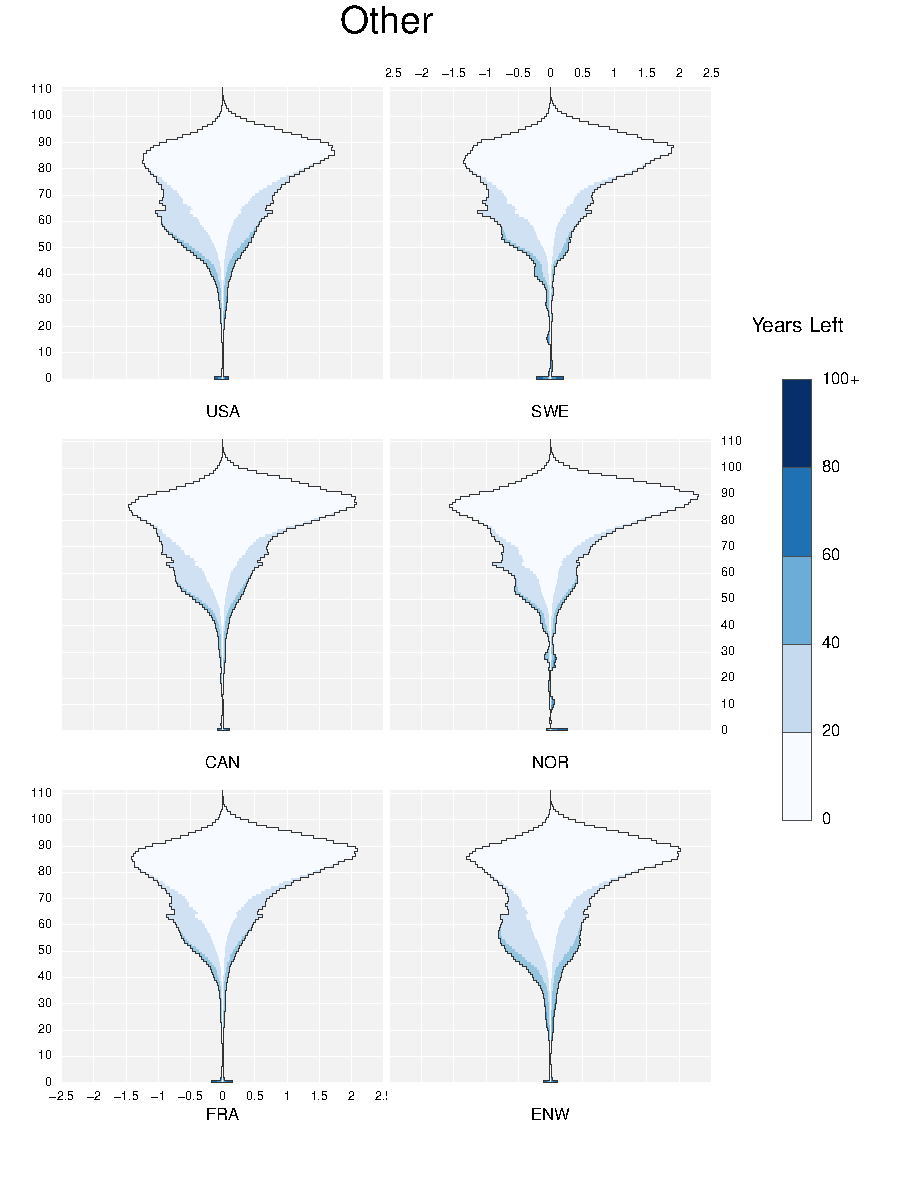
\includegraphics[scale=.8]{Figures/Causes/DxyOther.pdf}
%\end{figure}
%
%\pagebreak
%\subsection{$D^s(y)$, decomposed as in Figure~\ref{fig:Dyac}}
%\begin{figure}
%\centering
%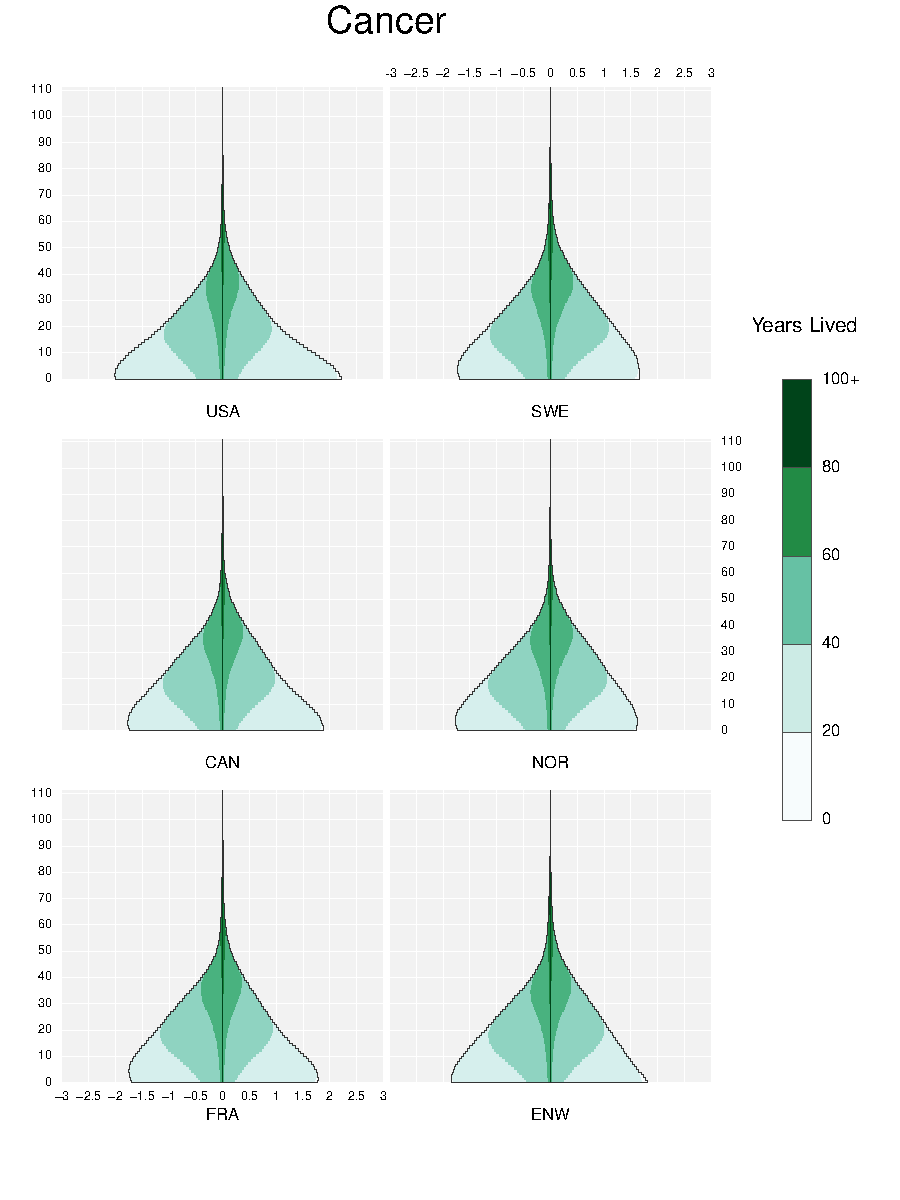
\includegraphics[scale=.8]{Figures/Causes/DyxCancer.pdf}
%\end{figure}
%\begin{figure}
%\centering
%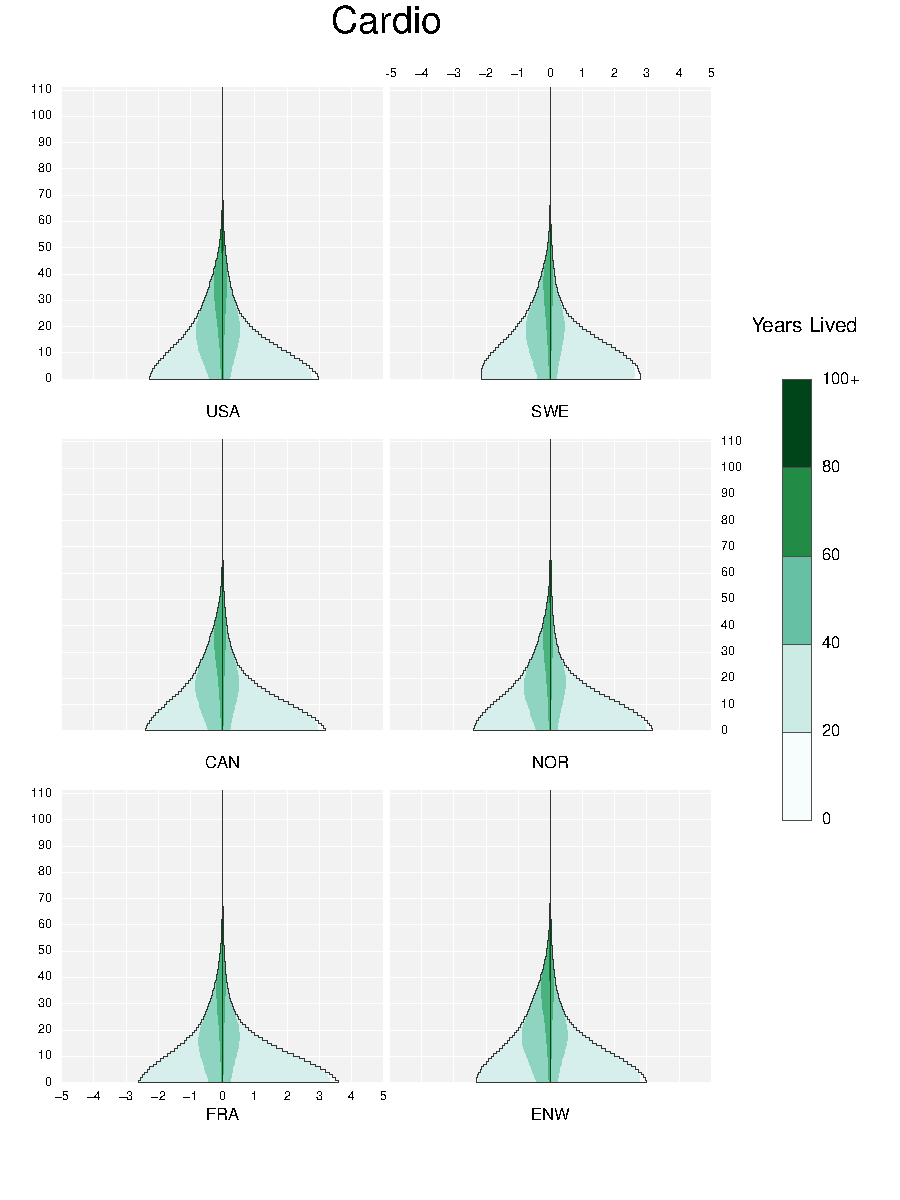
\includegraphics[scale=.8]{Figures/Causes/DyxCardio.pdf}
%\end{figure}
%\begin{figure}
%\centering
%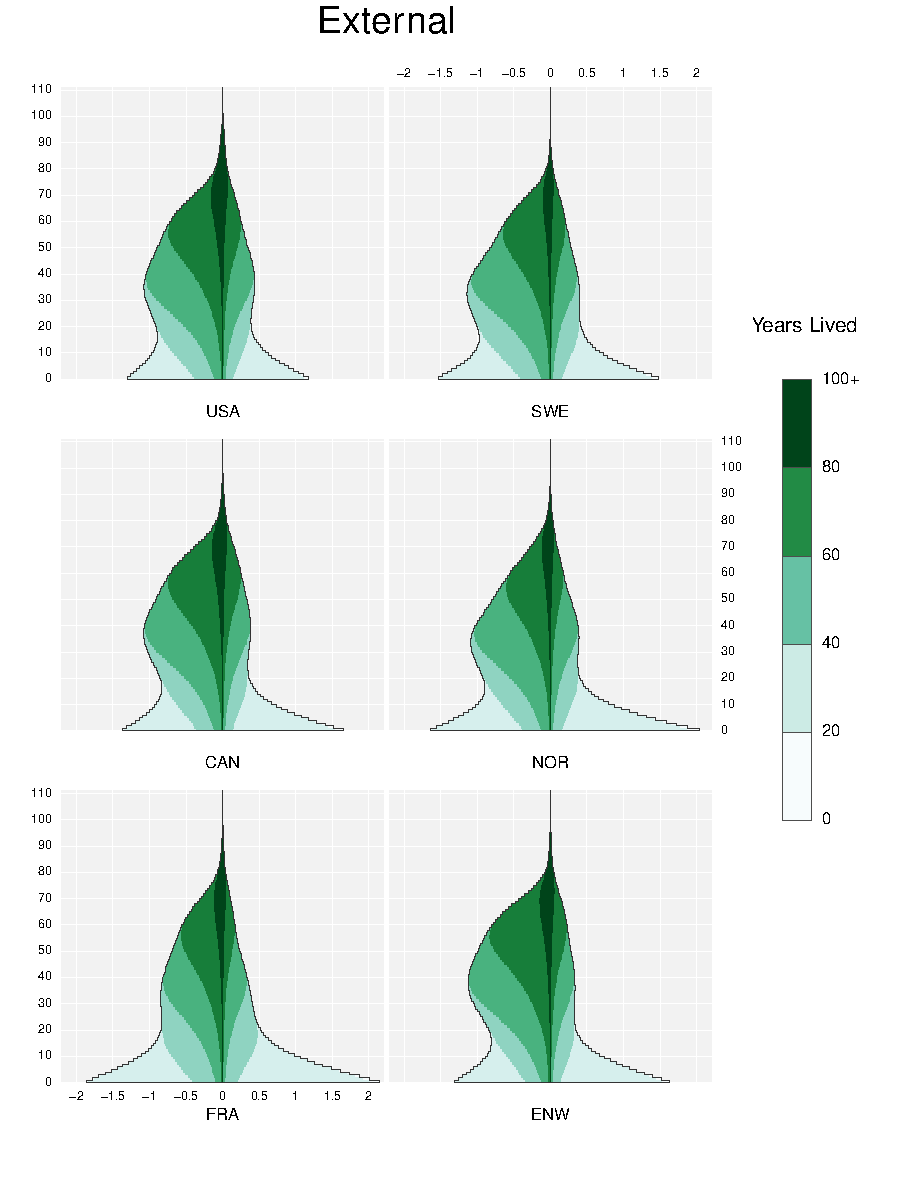
\includegraphics[scale=.8]{Figures/Causes/DyxExternal.pdf}
%\end{figure}
%\begin{figure}
%\centering
%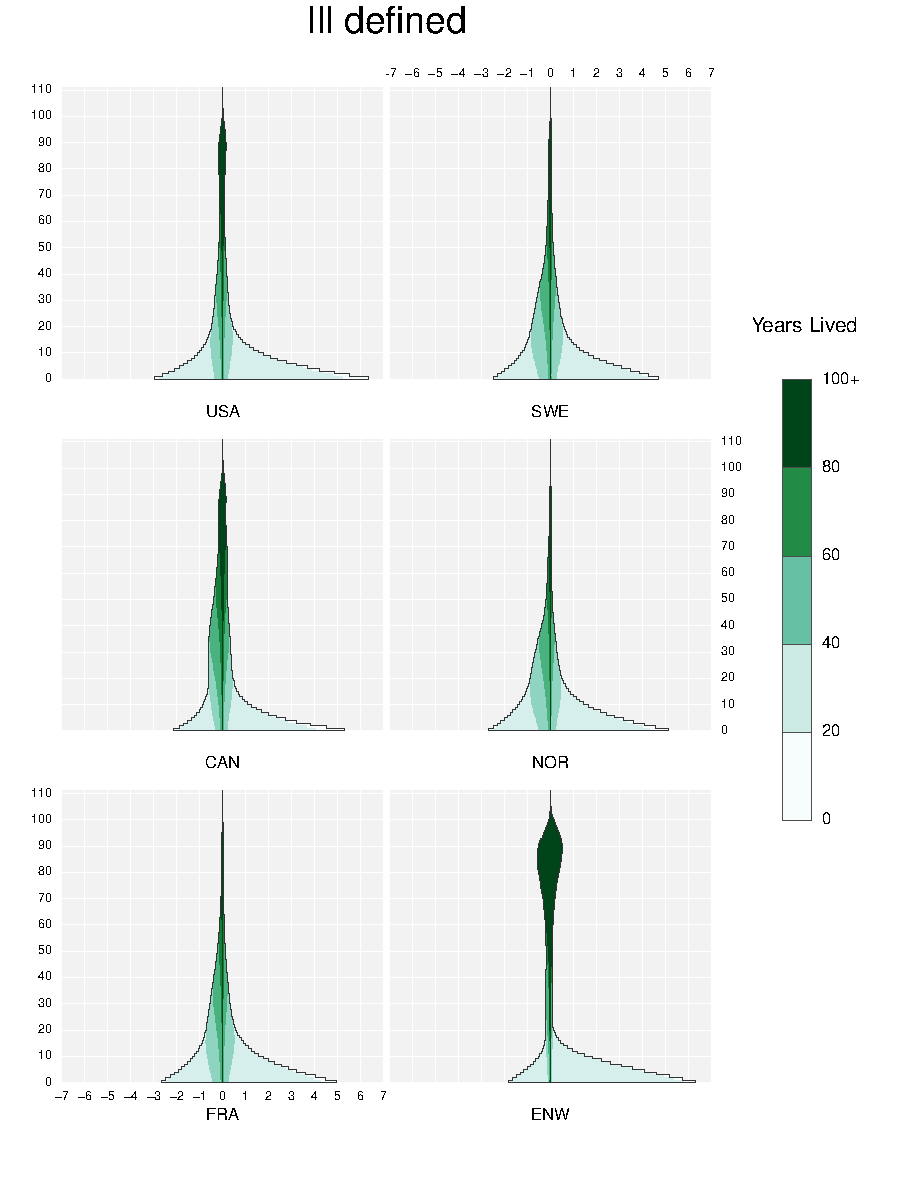
\includegraphics[scale=.8]{Figures/Causes/DyxIll defined.pdf}
%\end{figure}
%\begin{figure}
%\centering
%\includegraphics[scale=.8]{Figures/Causes/DyxInf_Cong.pdf}
%\end{figure}
%\begin{figure}
%\centering
%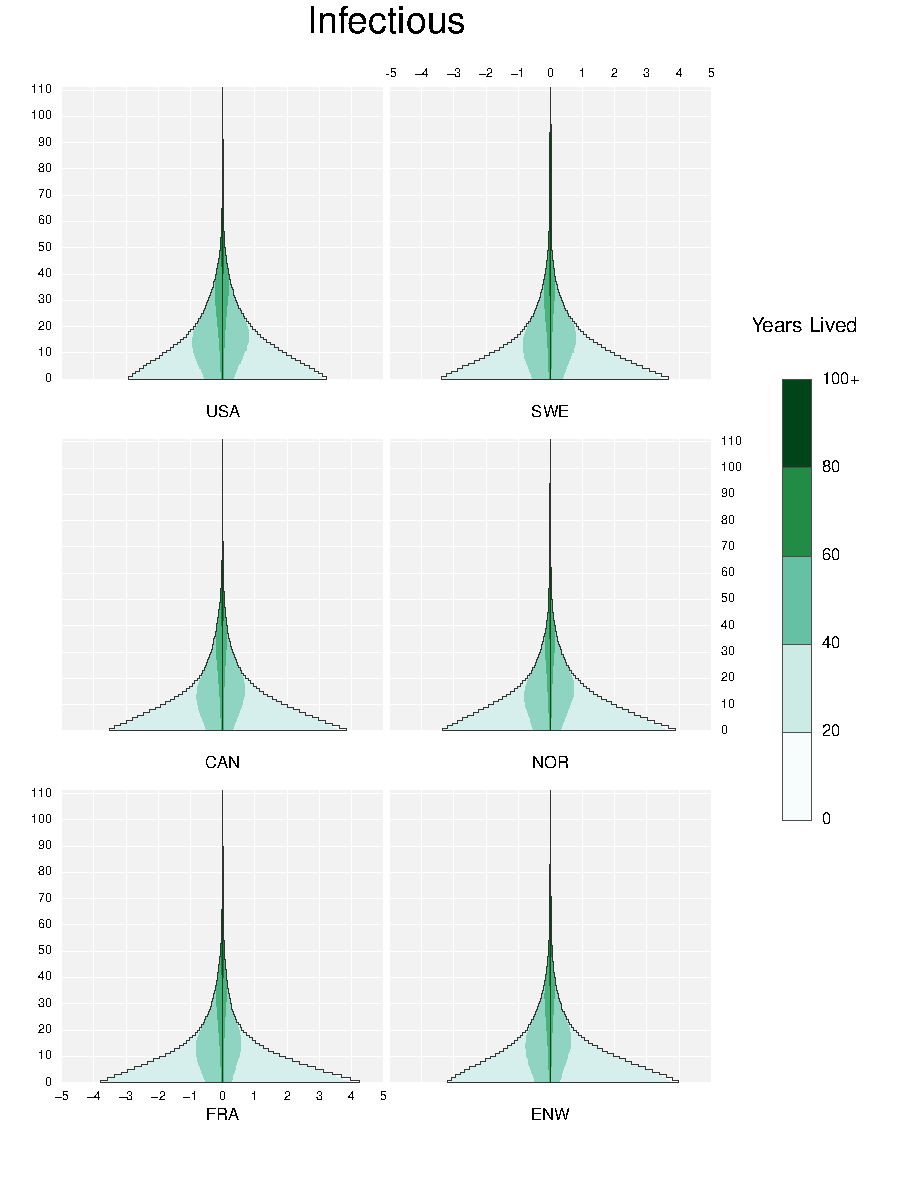
\includegraphics[scale=.8]{Figures/Causes/DyxInfectious.pdf}
%\end{figure}
%\begin{figure}
%\centering
%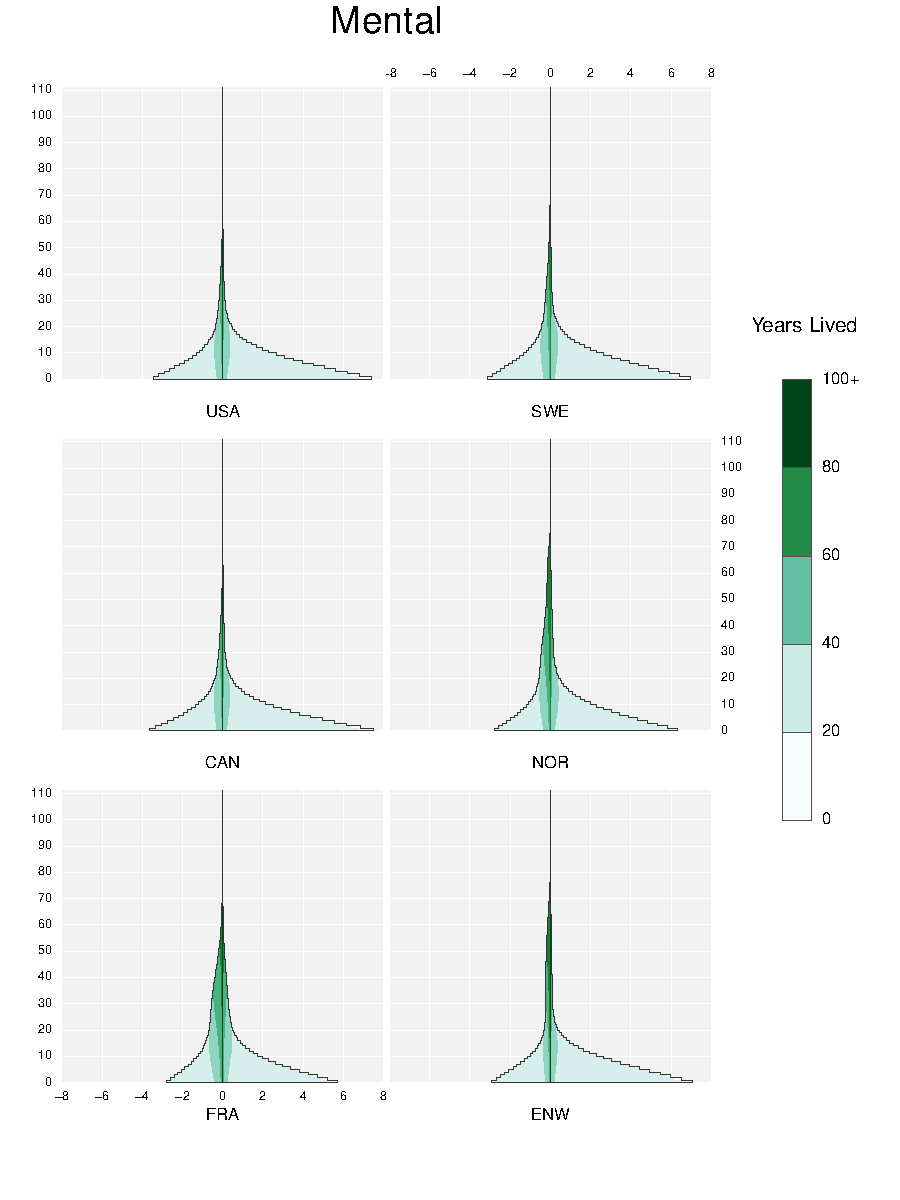
\includegraphics[scale=.8]{Figures/Causes/DyxMental.pdf}
%\end{figure}
%\begin{figure}
%\centering
%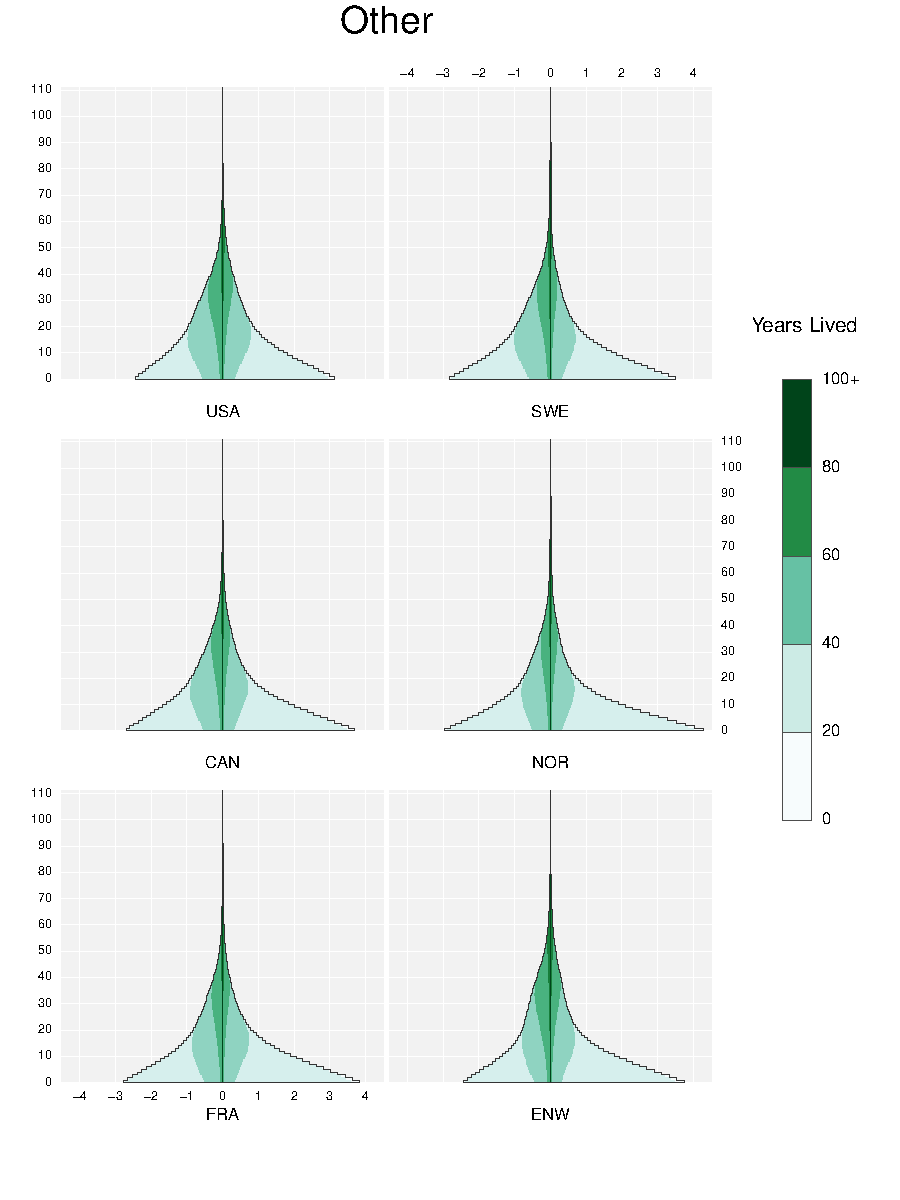
\includegraphics[scale=.8]{Figures/Causes/DyxOther.pdf}
%\end{figure}
%
%\pagebreak
%\subsection{$W^s(a)$, decomposed as in Figure~\ref{fig:SavedGainedUSAExternal}}
%FYI, Ill-defined casues are shown twice because the axes are strange. There are
%possibly coding issues going on here. Anyway, we needn't show it for the paper.
%Also, infant and congenital conditions are shown here, but on an x scale that is
%shrunk- msot of the mass is on age 0- instead we see the profile of higher ages,
%very choppy in this case (the empty ages in SWE and NOR were 0s in the original
%abridged data, and these have been maintained after graduation).
%\begin{figure}
%\centering
%\includegraphics[scale=.8]{Figures/Causes/WaCancer.pdf}
%\end{figure}
%\begin{figure}
%\centering
%\includegraphics[scale=.8]{Figures/Causes/WaCardio.pdf}
%\end{figure}
%\begin{figure}
%\centering
%\includegraphics[scale=.8]{Figures/Causes/WaExternal.pdf}
%\end{figure}
%%\begin{figure}
%%\centering
%%\includegraphics[scale=.8]{Figures/Causes/WaIll defined_1.pdf}
%%\end{figure}
%%\begin{figure}
%%\centering
%%\includegraphics[scale=.8]{Figures/Causes/WaIll defined_2.pdf}
%%\end{figure}
%\begin{figure}
%\centering
%\includegraphics[scale=.8]{Figures/Causes/WaInf_Cong.pdf}
%\end{figure}
%\begin{figure}
%\centering
%\includegraphics[scale=.8]{Figures/Causes/WaInfectious.pdf}
%\end{figure}
%\begin{figure}
%\centering
%\includegraphics[scale=.8]{Figures/Causes/WaMental.pdf}
%\end{figure}
%\begin{figure}
%\centering
%\includegraphics[scale=.8]{Figures/Causes/WaOther.pdf}
%\end{figure}
%
%\pagebreak
%\subsection{$W^s(a+y|a)$, decomposed as in
%Figure~\ref{fig:LostLivedUSAExternal}}
%\begin{figuAre}
%\centering
%\includegraphics[scale=.8]{Figures/Causes/WapygaCancer.pdf}
%\end{figure}
%\begin{figure}
%\centering
%\includegraphics[scale=.8]{Figures/Causes/WapygaCardio.pdf}
%\end{figure}
%\begin{figure}
%\centering
%\includegraphics[scale=.8]{Figures/Causes/WapygaExternal.pdf}
%\end{figure}
%\begin{figure}
%\centering
%\includegraphics[scale=.8]{Figures/Causes/WapygaIll defined.pdf}
%\end{figure}
%\begin{figure}
%\centering
%\includegraphics[scale=.8]{Figures/Causes/WapygaInf_Cong.pdf}
%\end{figure}
%\begin{figure}
%\centering
%\includegraphics[scale=.8]{Figures/Causes/WapygaInfectious.pdf}
%\end{figure}
%\begin{figure}
%\centering
%\includegraphics[scale=.8]{Figures/Causes/WapygaMental.pdf}
%\end{figure}
%\begin{figure}
%\centering
%\includegraphics[scale=.8]{Figures/Causes/WapygaOther.pdf}
%\end{figure}
%
\end{appendices}
\end{document}